\tikzset{every picture/.style={line width=0.75pt}} %set default line width to 0.75pt

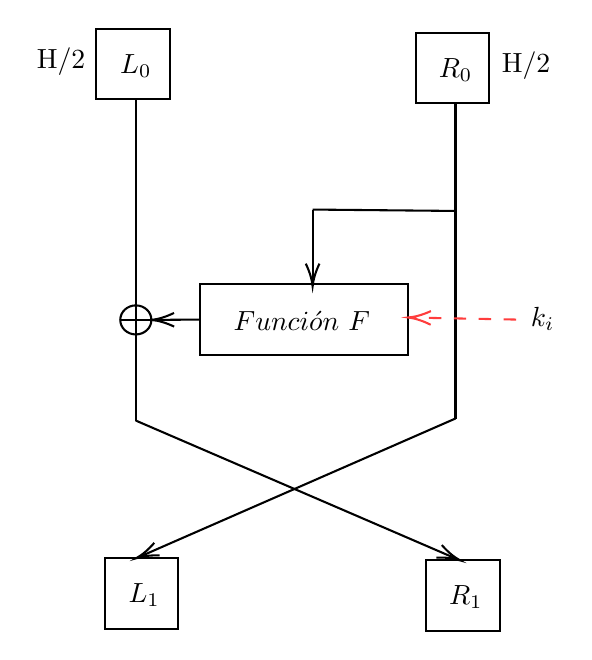
\begin{tikzpicture}[x=0.75pt,y=0.75pt,yscale=-1,xscale=1]
%uncomment if require: \path (0,607.4630661010742); %set diagram left start at 0, and has height of 607.4630661010742

%Shape: Rectangle [id:dp9387047590057875]
\draw   (124,32.2) -- (159.3,32.2) -- (159.3,66.2) -- (124,66.2) -- cycle ;
%Shape: Rectangle [id:dp06134354038145262]
\draw   (278,34.2) -- (313.3,34.2) -- (313.3,68.2) -- (278,68.2) -- cycle ;
%Straight Lines [id:da10790130820156896]
\draw    (143,66.5) -- (143,165.5) ;


%Flowchart: Or [id:dp07980698217083693]
\draw   (135.5,172.5) .. controls (135.5,168.63) and (138.86,165.5) .. (143,165.5) .. controls (147.14,165.5) and (150.5,168.63) .. (150.5,172.5) .. controls (150.5,176.37) and (147.14,179.5) .. (143,179.5) .. controls (138.86,179.5) and (135.5,176.37) .. (135.5,172.5) -- cycle ; \draw   (135.5,172.5) -- (150.5,172.5) ; \draw   (143,165.5) -- (143,179.5) ;
%Shape: Rectangle [id:dp9005647886302468]
\draw   (174,155.2) -- (274,155.2) -- (274,189.2) -- (174,189.2) -- cycle ;

%Shape: Rectangle [id:dp1446172377376469]
\draw   (128,287.2) -- (163.3,287.2) -- (163.3,321.2) -- (128,321.2) -- cycle ;
%Shape: Rectangle [id:dp5944788483468033]
\draw   (283,288.2) -- (318.3,288.2) -- (318.3,322.2) -- (283,322.2) -- cycle ;
%Straight Lines [id:da5126430845478047]
\draw    (297,68.5) -- (297,220) ;


%Straight Lines [id:da8558270544869495]
\draw    (143,179.5) -- (143,221) ;


%Straight Lines [id:da15557753762708693]
\draw    (143,221) -- (297.33,287.54) ;
\draw [shift={(299.17,288.33)}, rotate = 203.32] [color={rgb, 255:red, 0; green, 0; blue, 0 }  ][line width=0.75]    (10.93,-3.29) .. controls (6.95,-1.4) and (3.31,-0.3) .. (0,0) .. controls (3.31,0.3) and (6.95,1.4) .. (10.93,3.29)   ;

%Straight Lines [id:da21080378203535233]
\draw    (297,220) -- (145,286.53) ;
\draw [shift={(143.17,287.33)}, rotate = 336.36] [color={rgb, 255:red, 0; green, 0; blue, 0 }  ][line width=0.75]    (10.93,-3.29) .. controls (6.95,-1.4) and (3.31,-0.3) .. (0,0) .. controls (3.31,0.3) and (6.95,1.4) .. (10.93,3.29)   ;

%Straight Lines [id:da7320888588354941]
\draw    (228.17,119.33) -- (228.17,154.33) ;
\draw [shift={(228.17,156.33)}, rotate = 270] [color={rgb, 255:red, 0; green, 0; blue, 0 }  ][line width=0.75]    (10.93,-3.29) .. controls (6.95,-1.4) and (3.31,-0.3) .. (0,0) .. controls (3.31,0.3) and (6.95,1.4) .. (10.93,3.29)   ;

%Straight Lines [id:da6084690526516647]
\draw    (228.17,119.33) -- (297,120) ;


%Straight Lines [id:da29161126742281174]
\draw [color={rgb, 255:red, 255; green, 61; blue, 61 }  ,draw opacity=1 ] [dash pattern={on 4.5pt off 4.5pt}]  (326.17,172.33) -- (276.17,171.37) ;
\draw [shift={(274.17,171.33)}, rotate = 361.1] [color={rgb, 255:red, 255; green, 61; blue, 61 }  ,draw opacity=1 ][line width=0.75]    (10.93,-3.29) .. controls (6.95,-1.4) and (3.31,-0.3) .. (0,0) .. controls (3.31,0.3) and (6.95,1.4) .. (10.93,3.29)   ;

%Straight Lines [id:da9288138682659981]
\draw    (174.17,172.33) -- (152.5,172.49) ;
\draw [shift={(150.5,172.5)}, rotate = 359.6] [color={rgb, 255:red, 0; green, 0; blue, 0 }  ][line width=0.75]    (10.93,-3.29) .. controls (6.95,-1.4) and (3.31,-0.3) .. (0,0) .. controls (3.31,0.3) and (6.95,1.4) .. (10.93,3.29)   ;


% Text Node
\draw (143,50) node  [align=left] {$\displaystyle L_{0}$};
% Text Node
\draw (297,52) node  [align=left] {$\displaystyle R_{0}$};
% Text Node
\draw (223,173) node  [align=left] {$\displaystyle Funci\acute{o}n\ F$};
% Text Node
\draw (147,305) node  [align=left] {$\displaystyle L_{1}$};
% Text Node
\draw (302,306) node  [align=left] {$\displaystyle R_{1}$};
% Text Node
\draw (339,172) node  [align=left] {$\displaystyle k_{i}$};
% Text Node
\draw (107,48) node  [align=left] {H/2};
% Text Node
\draw (331,50) node  [align=left] {H/2};


\end{tikzpicture}